\section{Colouring classes}\label{sec:colouring-classes}

It is now possible to visualize all possible colouring sets of proper (2,3)-poles on their colouring graphs. Since there is no rule on which semiedges are labelled $b_1,b_2,b_3$ after removing a vertex from a snark, we will divide the colouring sets into classes, in which the colouring sets represent isomorphic colourings up to the~choice of labelling $b_1,b_2,b_3$.

However, not each graph on these vertices represents a possible colouring set. First, the graph must have no pendant vertex, as was proven above. The second restriction is that no edge is between two vertices from $\{b_1,b_2,b_3\}$. Suppose there was an edge between $b_1$ and $b_2$ in any proper (2,3)-pole $T$. This would mean that $T$ allows a colouring such that $b_1,b_2$ and $b_3$ have pairwise different colours and $a_1,a_2$ have the same colour. Thus $T$ could be extended to the former graph, which would be colourable and therefore not a snark, which contradicts the assumption.

This means there are only $12$ different colouring sets of proper (2,3)-poles, which can be divided into classes in the following way. We denote the classes by a number representing how many vertices from $\{b_1,b_2,b_3\}$ are connected to $\{a_1,a_2\}$ with an edge in the colouring graph, followed by A if the colouring allows an edge between $a_1$ and $a_2$, or B otherwise. Resulting are six colouring classes: 0B (uncolourable), 1A, 2B, 2A, 3B and 3A (perfect). For each of them we have found an example, in this article we provide an example of an uncolourable proper (2,3)-pole in \cref{fig:uncolourable-example} resulting from the second Blanuša snark and a perfect one in \cref{fig:perfect-example} resulting from the Petersen graph.

\begin{figure}
	\centering
	\scalebox{0.7}{
		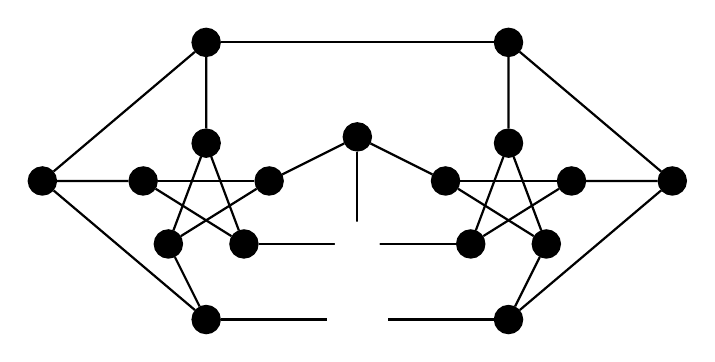
\begin{tikzpicture}[scale=0.8, every node/.style={draw,circle,very thick,fill=black}]
	\node (0) at (-2.4, 4.9) {};
	\node (1) at (0, 1.7) {};
	\node (2) at (-3, 1.7) {};
	\node (3) at (-3.4, 2.7) {};
	\node (4) at (-2.4, 3.3) {};
	\node (5) at (-1.8, 1.7) {};
	\node (6) at (0, 3.4) {};
	\node (7) at (-1.4, 2.7) {};
	\node (8) at (-5, 2.7) {};
	\node (9) at (-2.4, 0.5) {};
	\node (10) at (3, 1.7) {};
	\node (11) at (2.4, 0.5) {};
	\node (12) at (2.4, 4.9) {};
	\node (13) at (5, 2.7) {};
	\node (14) at (1.8, 1.7) {};
	\node (15) at (2.4, 3.3) {};
	\node (16) at (1.4, 2.7) {};
	\node (17) at (3.4, 2.7) {};
	
	\path[draw, thick]
	(0) edge (4) 
	(0) edge (8) 
	(0) edge (12) 
	(1) edge (5) 
	(1) edge (6) 
	(1) edge (14) 
	(2) edge (4) 
	(2) edge (7) 
	(2) edge (9) 
	(3) edge (5) 
	(3) edge (7) 
	(3) edge (8) 
	(4) edge (5) 
	(6) edge (7) 
	(6) edge (16) 
	(8) edge (9) 
	%(9) edge (11) 
	(10) edge (11) 
	(10) edge (15) 
	(10) edge (16) 
	(11) edge (13) 
	(12) edge (13) 
	(12) edge (15) 
	(13) edge (17) 
	(14) edge (15) 
	(14) edge (17) 
	(16) edge (17) 
	
	(9) edge  ++(1.92, 0)
	(11) edge ++ (-1.92, 0)
	;
	
	\node at (1) [draw=white,fill=white, minimum size=1.5em] {};
\end{tikzpicture}
	}
	\caption{Example of an uncolourable proper (2,3)-pole}
	\label{fig:uncolourable-example}
\end{figure}

\begin{figure}
	\centering
	\begin{tikzpicture}[every node/.style={draw,circle,very thick,fill=black}]
	\graph[clockwise, radius=2cm, empty nodes] {subgraph I_n [n=5,name=A, V={1,2,3,4,5}] };
	\graph[clockwise, radius=1cm, empty nodes] {subgraph I_n [n=5,name=B, V={1,2,3,4,5}] };
	
	\draw (B 1) -- (B 3);
	\draw (B 3) -- (B 5);
	\draw (B 5) -- (B 2);
	\draw (B 2) -- (B 4);
	\draw (B 4) -- (B 1);
	
	\draw (A 1) -- (B 1);
	\draw (A 2) -- (B 2);
	\draw (A 3) -- (B 3);
	\draw (A 4) -- (B 4);
	\draw (A 5) -- (B 5);
	
	\draw (A 1) -- (A 2);
	\draw (A 2) -- (A 3);
	%\draw (A 3) -- (A 4);
	\draw (A 4) -- (A 5);
	\draw (A 5) -- (A 1);
	
	\draw (A 3) -- ++(0,-1);
	\draw (A 4) -- ++(0,-1);
	
	\node at (B 1) [draw=white,fill=white, circle, very thick, minimum size=1.2em] {};
\end{tikzpicture}
	\caption{Example of a perfect proper (2,3)-pole}
	\label{fig:perfect-example}
\end{figure}